\documentclass[10pt,a4paper]{article}
\usepackage[paper=a4paper, hmargin=1.5cm, bottom=1.5cm, top=3cm]{geometry}

\usepackage[utf8x]{inputenc}
\usepackage[spanish]{babel}

\usepackage{mathtools}
\usepackage{amsmath}
\usepackage{amsfonts}
\usepackage{amssymb}

\usepackage{xcolor}
\usepackage{listingsutf8}
\usepackage{booktabs}
\usepackage{hyperref}
\usepackage{multirow}

\usepackage{caption}
\usepackage{subcaption}

\usepackage{algorithm}
\usepackage[noend]{algpseudocode}

\usepackage{graphicx}
\usepackage{tikz}
\usepackage{relsize}

\usepackage{chessboard}
\storechessboardstyle{6x6}{maxfield=h8}

\DeclarePairedDelimiter{\ceil}{\lceil}{\rceil}

%\let\NombreFuncion=\textsc
%\let\TipoVariable=\texttt

%\newcommand{\TipoFuncion}[3]{%
  %\NombreFuncion{#1}(#2) \ifx#3\empty\else $\to$ \res\,: \TipoVariable{#3}\fi%
%}

% set the default code style
\lstset{
    frame=tb, % draw a frame at the top and bottom of the code block
    tabsize=4, % tab space width
    showstringspaces=false, % don't mark spaces in strings
    numbers=left, % display line numbers on the left
    commentstyle=\color{green}, % comment color
    keywordstyle=\color{blue}, % keyword color
    stringstyle=\color{red} % string color
}

% mathy stuff
\newtheorem{theorem}{Theorem}[section]
\newtheorem{lemma}[theorem]{Lemma}
\newtheorem{proposition}[theorem]{Proposición}
\newtheorem{corollary}[theorem]{Corollary}

\newenvironment{proof}[1][Demostración]{\begin{trivlist}
\item[\hskip \labelsep {\bfseries #1}]}{\end{trivlist}}
\newenvironment{definition}[1][Definición]{\begin{trivlist}
\item[\hskip \labelsep {\bfseries #1}]}{\end{trivlist}}
\newenvironment{example}[1][Example]{\begin{trivlist}
\item[\hskip \labelsep {\bfseries #1}]}{\end{trivlist}}
\newenvironment{remark}[1][Remark]{\begin{trivlist}
\item[\hskip \labelsep {\bfseries #1}]}{\end{trivlist}}

\newcommand{\qed}{\nobreak \ifvmode \relax \else
      \ifdim\lastskip<1.5em \hskip-\lastskip
      \hskip1.5em plus0em minus0.5em \fi \nobreak
      \vrule height0.75em width0.5em depth0.25em\fi}

\title{Sistemas Operativos \\ TP1}

\newcommand{\order}[1]{$\mathcal{O}(#1)$}

\begin{document}

%% cover page

\maketitle

\bigskip

\begin{table}[h]
\centering
\begin{tabular}{|l l l|}
\hline
Integrante       & \multicolumn{1}{c}{LU}     & Correo electrónico        \\ \hline
Martin Baigorria & \multicolumn{1}{c}{575/14} & martinbaigorria@gmail.com \\ 
Federico Beuter & 827/13                      & federicobeuter@gmail.com \\
Rodrigo Kapobel & 864/13                      & jangamesdev@gmail.com \\ 
Mauro Cherubini & 835/13                      & cheru.mf@gmail.com \\ \hline
\end{tabular}
\end{table}

\vfill

\begin{center}
\textbf{Reservado para la cátedra}
\end{center}
\begin{table}[h]
\centering
\begin{tabular}{|l|l|l|}
\hline
Instancia       & Docente & Nota \\ \hline
Primera entrega &         &      \\ \hline
Segunda entrega &         &      \\ \hline
\end{tabular}
\end{table}

\newpage
\tableofcontents
\newpage

% end cover page

\section{Task Consola}

En este ejercicio programamos la tarea \texttt{Task Consola}, que lo que hace es simular una tarea interactiva que realiza $n$ llamadas bloqueantes con una duración de ticks de reloj aleatoria entre \texttt{bmin} y \texttt{bmax}.

Una llamada se clasifica como \texttt{bloqueante} cuando el procesador no puede seguir ejecutando instrucciones hasta que algun tipo de recurso este disponible. Las llamadas bloqueantes en general son de entrada y salida. Este tipo de recursos se acceden comunmanete mediante un \texttt{syscall}. El \texttt{syscall} en si debe ser ejecutado en primera instancia, lo que asumiremos que toma un ciclo de reloj. Luego el recurso toma un total de $t$ ticks de reloj de forma aleatoria en responder. Por lo tanto, una tarea ineractiva toma un ciclo de reloj para la llamada y permanecera bloqueada durante $t$ ciclos adicionales.

\subsection{Código}

\begin{lstlisting}[language=C++, breaklines=true]
void TaskConsola(int pid, vector<int> params) {
	srand(1); // set seed

	for (int i = 0; i < params[0]; ++i) {
		int t = params[1] + rand() % (params[2] - params[1] + 1);
		uso_IO(pid, t);
	}
}
\end{lstlisting}

Esta tarea toma un \texttt{pid} y un vector \texttt{params} de 3 parámetros. Dado que nuestros resultados dependerán de un generador de números pseudo-aleatorio, setteamos una semilla con el objetivo de poder replicar nuestros resultados.

Luego, el loop ejecuta la llamada \texttt{bloqueante} simulada con un request de entrada/salida utilizando como parámetro un numero aleatorio entre \texttt{bmin} y \texttt{bmax} que se encuentran en el vector en ese orden respectivamente.

Este numero no necesariamente tiene una distribución uniforme perfecta, pero se le parece demasiado dado que genera un valor entre $0$ y \texttt{RAND\_MAX}\footnote{http://www.cplusplus.com/reference/cstdlib/RAND\_MAX} (definido en la std) y luego le aplica la función modulo con un numero chico a un dominio grande. La función devuelve un numero $t \in [0, RAND\_MAX]$. La función modulo luego achica ese dominio a $[0, bmax - bmin]$. Finalmente, al sumarle bmin logramos que $t \in [bmin, bmax]$.

\subsubsection{Diagrama GANTT}

El siguiente diagrama fue generado con los siguientes parametros:

\begin{enumerate}
	\item lote\_tsk: 1.tsk
	\item num\_cores: 1
	\item switch\_cost: 0
	\item sched\_class: SchedFCFS
	\item n: 10
	\item bmin: 1
	\item bmax: 10
\end{enumerate}

\begin{figure}[h]
    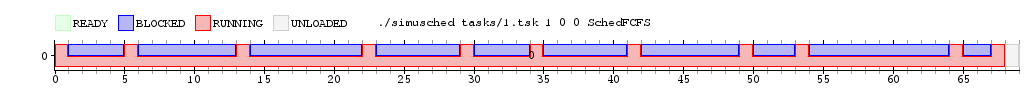
\includegraphics[width=\linewidth]{images/1.png}
    \label{fig:Task Consola}
    \caption{Task Consola}
\end{figure}

\textbf{TODO: Explicar bien el diagrama!}
\newpage
\section{Rolando}

\subsection{Diagrama GANTT}

El siguiente diagrama fue generado con los siguientes parametros:

\begin{enumerate}
	\item lote\_tsk: 2.tsk
	\item num\_cores: 1
	\item switch\_cost: 4
	\item sched\_class: SchedFCFS
\end{enumerate}

\begin{figure}[h]
    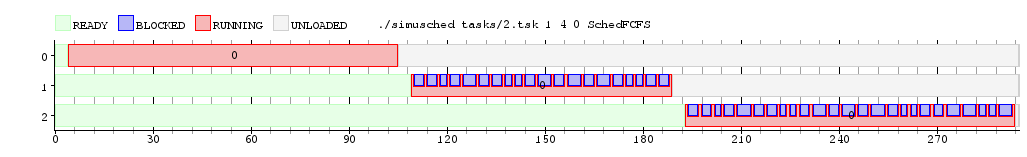
\includegraphics[width=\linewidth]{images/2_1nucleo.png}
    \label{fig:Task Consola}
    \caption{Rolando con 1 núcleo}
\end{figure}

En la figura 2 se presenta el diagrama de Gantt del \textit{lote2} bajo el algortimo del scheduler FCFS. Este lote simula la situaci\'on de \textit{Rolando}, para el que se requiere ejecutar 3 tareas. Las tres tendr\'an un \textit{release time} nulo, de modo que cada tarea s\'olo deber\'a esperar al costo de cambio de contexto para entrar en estado \textit{runing}. La primera, que es del tipo TaskCPU y con su parametro igual a 100, tras esperar 4 ciclos de reloj (por el \textit{switch\_cost}), como su parametro indica, hace uso del CPU durante 100 ciclos de rejoj, y uno extra por la llamada a \textit{exit()}. Tras finalizar la anterior, y despu\'es de otros 4 ciclos por el cambio de contexto, pasa al estado \textit{runing} la segunda tarea, esta vez de tipo TaskConsola y con el vector \textit{$<$20, 2, 4$>$} como parametro. Esta efectua 20 llamadas bloqueantes, que demoran entre 2 a 4 ciclos, haciendo uso de 20 llamadas consecutivas a \textit{uso\_IO()} que requieren a su vez de 1 ciclo cada una. Por \'ultimo, luego de emplear su \'ultimo ciclo asignado para llamar a \textit{exit()}, y tras demorarse otros 4 por el cambio de contexto, pasa al estado \textit{runing} la \'ultima tarea del lote. Nuevamente es del tipo TaskConsola, esta vez con el vector \textit{$<$25, 2, 4$>$} como parametro. De igual manera que en la tarea anterior se hace uso de \textit{uso\_IO()} para efectuar las 25 llamadas bloqueantes, y de \textit{exit()} en el \'ultimo ciclo.

\begin{enumerate}
	\item lote\_tsk: 2.tsk
	\item num\_cores: 2
	\item switch\_cost: 4
	\item sched\_class: SchedFCFS
\end{enumerate}

\begin{figure}[h]
    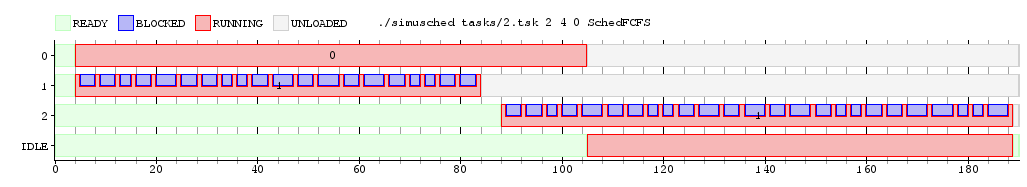
\includegraphics[width=\linewidth]{images/2_2nucleos.png}
    \label{fig:Task Consola}
    \caption{Rolando con 2 núcleos}
\end{figure}

En la Figura 3 se observa el diagrama de Gantt del mismo lote de tareas y scheduler de antes, pero esta vez bajo una CPU que cuenta con dos nucleos. Al igual que el caso anterior, el \textit{switch\_cost}) es de 4 ciclos, por lo que se demora esta cantidad de tiempo empezar a correr la primera tarea. Que a diferencia del caso anterior (en el que se contaba con un s\'olo nucleo) tras ese tiempo, pasan al estado \textit{runing} las primeras 2 tareas (una en cada nucleo). Trabajando como se explico en el caso anterior, luego de terminar la tarea asignada al \textit{label} 1 del grafico (la TaskConsola 20 2 4), pasa al estado \textit{runing} la \'ultima tarea restante  
\newpage
\section{TaskBatch}

\subsection{Código}

\begin{lstlisting}[language=C++, breaklines=true]
void TaskBatch(int pid, vector<int> params) {

	srand(1); // set seed

	int total_cpu = params[0];
	int cant_bloqueos = params[1];

	bool config[total_cpu];
	fill_n(config, total_cpu, false);
	for (int i = 0; i < cant_bloqueos; i++) config[i] = true;
	random_shuffle(&config[0], &config[total_cpu-1]);

	for (int i = 0; i < total_cpu; ++i) {
		if (config[i] == true) { // block
			uso_IO(pid, 1);
		} else {
			uso_CPU(pid, 1);
		}
	}
}
\end{lstlisting}

El codigo que simula la tarea \texttt{TaskBatch} recibe dos parametros, estos son la cantidad de total de ciclos de reloj que lleva ejecutar la tarea y la cantidad de llamadas bloqueantes que ocurriran durante la ejecucion de la misma. A partir de la cantidad total de ciclos de CPU, se arma un vector en donde van a estar colocados los momentos donde ocurra una llamada bloqueante, estos se colocan de manera pseudoaleatoria con la funcion \texttt{random\_shuffle}. Una vez que termine este proceso, procedemos a simular la ejecucion de los ciclos de CPU utilizando el vector, si este indica que se debe producir una llamada bloqueante hace una llamada a \texttt{uso\_IO}, en el caso contrario se ejecuta un ciclo de CPU.

\subsubsection{Diagrama GANTT}

El siguiente diagrama fue generado con los siguientes parametros:

\begin{enumerate}
	\item lote\_tsk: 3.tsk
	\item num\_cores: 1
	\item switch\_cost: 1
	\item sched\_class: SchedFCFS
\end{enumerate}

\begin{figure}[h]
    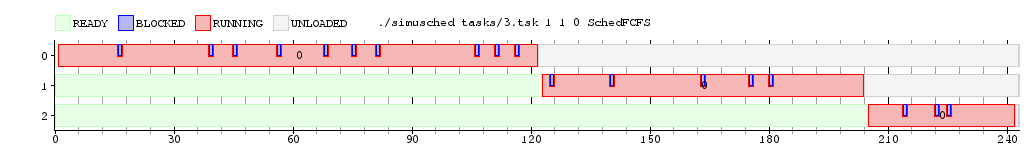
\includegraphics[width=\linewidth]{images/3.png}
    \label{fig:Task Consola}
    \caption{Task Batch}
\end{figure}

En la figura 4 tenemos el diagrama de Gantt de la ejecucion de tareas del lote 3, las tareas ejecutadas en el mismo cumplen con los siguientes parametros:

\begin{itemize}
	\item Tarea 0: 100 ciclos de CPU, 10 llamadas bloqueantes
	\item Tarea 1: 70 ciclos de CPU, 5 llamadas bloqueantes
	\item Tarea 2: 30 ciclos de CPU, 3 llamadas bloqueantes
\end{itemize}

Como podemos apreciar, el diagrama cumple perfectamente con el scheduler FCFS, es decir, las tareas no son desalojadas y se las mantiene en ejecucion hasta que concluyan. Ademas podemos ver que el diagrama respeta el costo de hacer una llamada bloqueante, tomando un ciclo adicional antes de efectuar las mismas.
\newpage
\section{Round Robin Implementation}

\subsection{Código}

En primer lugar, modificamos la declaracion de la clase  \texttt{SchedRR} agregando una serie de atributos privados:

\subsubsection{Class Declaration}
\begin{lstlisting}[language=C++, breaklines=true]
class SchedRR : public SchedBase {
	public:
		SchedRR(std::vector<int> argn);
        ~SchedRR();
		virtual void load(int pid);
		virtual void unblock(int pid);
		virtual int tick(int cpu, const enum Motivo m);

	private:
		int* quantum;
		int* cycles;
		std::queue<int> q;
};
\end{lstlisting}

Por un lado, el puntero de enteros llamado \texttt{quantum} nos dice por cuantos ciclos de clock nuestras tareas se van a ejecutar por CPU. Por otro lado, tenemos un puntero de enteros llamado \texttt{cycles}, que lo que hace es mantener la cuenta de cuantos ciclos le quedan a cada tarea en ejecución por CPU antes de llegar al quantum. Finalmente, tenemos una cola de tareas \texttt{q} compartida entre CPUs.

\subsubsection{Constructor y Destructor}
\begin{lstlisting}[language=C++, breaklines=true]
SchedRR::SchedRR(vector<int> argn) {
	// Round robin recibe la cantidad de cores y sus cpu_quantum por parametro
	quantum = new int[argn.size()-1];

	for (int i = 1; i < (int) argn.size(); i++) {
		quantum[i-1] = argn[i];
	}

	cycles = new int[argn[0]];
}
\end{lstlisting}

Aqui tenemos en \texttt{quantum} el arreglo del quantum por CPU, mientras que en \texttt{cycles} tenemos un arreglo que mantiene la cantidad de ciclos restantes del quantum de cada CPU.

\begin{lstlisting}[language=C++, breaklines=true]
SchedRR::~SchedRR() {
	delete[] cycles;
	delete[] quantum;
}
\end{lstlisting}

El destructor se encarga de liberar la memoria alocada por los dos arreglos.

\subsection{Load y Unblock}

\begin{lstlisting}[language=C++, breaklines=true]
void SchedRR::load(int pid) {
	q.push(pid);
}

void SchedRR::unblock(int pid) {
	q.push(pid);
}
\end{lstlisting}

Estas funciones se encargan de cargar tareas y de volverlas a cargar cuando se desbloquean. En este caso la implementacion es simple, ya que la migracion de procesos entre CPUs nos permite tener una unica cola, con lo cual alcanza con agregarlas a la misma para que entren en la rotacion de tareas.

\subsubsection{Tick}

Aqui tenemos el ciclo de ejecucion del $tick$ del scheduler, el mismo se encarga de manejar el desalojo de tareas:

\begin{lstlisting}[language=C++, breaklines=true]
int SchedRR::tick(int cpu, const enum Motivo m) {
	if (m == EXIT || m == BLOCK) {
		// Si el pid actual termino, sigue el proximo.
		if (q.empty()) return IDLE_TASK;
		else {
			int sig = q.front(); q.pop();
			cycles[cpu] = quantum[cpu];
			return sig;
		}
	} else {
		if (current_pid(cpu) == IDLE_TASK && !q.empty()) {
			int sig = q.front(); q.pop();
			cycles[cpu] = quantum[cpu];
			return sig;
		} else {
			cycles[cpu]--;

			if (cycles[cpu] == 0) {
				if (q.empty()) {
					cycles[cpu] = quantum[cpu];
					return current_pid(cpu);
				} else {
					int sig = q.front(); q.pop();
					q.push(current_pid(cpu)); // re-add to queue
					cycles[cpu] = quantum[cpu];
					return sig;
				}
			} else {
				return current_pid(cpu);
			}
		}
	}
}
\end{lstlisting}

Como podemos apreciar, primero se considera si la tarea actual ejecutandose en la CPU termino u ocurrio un bloqueo, en ambos casos se la desaloja y se la cambia por la siguiente tarea en la cola, resetando el quantum en el proceso. Si el procesador se encuantra ejecutando la tarea IDLE y hay tareas esperando a ser ejecutadas, se procede a ejecutar la primera que este en la cola y se resetea el quantum para la CPU. Si no se presentan ninguno de los dos casos anteriores, el scheduler chequea el quantum actual, si aun no termino se mantiene la tarea actual y se concluye el $tick$. En el caso que haya terminado el quantum se chequea la cola de tareas, si no hay tareas en espera se resetea el quantum, en el caso contrario se efectua el cambio de tarea con la primer tarea de la cola tambien reseteando el quantum.
\\
Para verificar la correcta implementacion de los mecanismos de $Round Robin$, tenemos la siguiente configuracion del scheduler:

\begin{enumerate}
	\item lote\_tsk: 2.tsk
	\item num\_cores: 2
	\item switch\_cost: 2
	\item sched\_class: SchedRR
	\item params: 5 10
\end{enumerate}

Esta configuracion fue usada durante el procesamiento del lote 4, que compone las siguientes tareas:

\begin{itemize}
	\item Tarea 0: 40 ciclos de CPU, 0 llamadas bloqueantes
	\item Tarea 1: 40 ciclos de CPU, 0 llamadas bloqueantes
	\item Tarea 2: 40 ciclos de CPU, 0 llamadas bloqueantes
	\item Tarea 3: 20 ciclos de CPU, 5 llamadas bloqueates, incorporada en el momento 10
\end{itemize}

El resultado obtenido fue el siguiente:

\begin{figure}[h]
    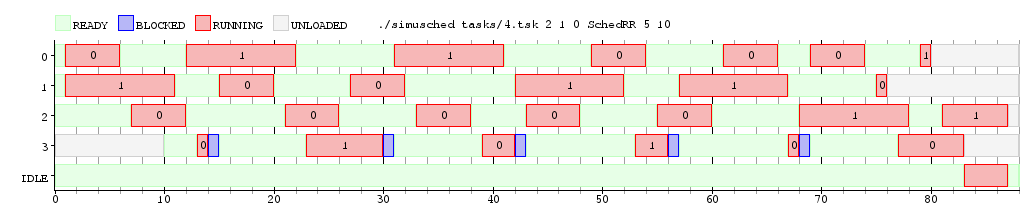
\includegraphics[width=\linewidth]{images/4.png}
    \label{fig:Task Consola}
    \caption{Task Batch}
\end{figure}

Como podemos apreciar en el grafico, cada uno de los \textit{Cores} tiene su propio quantum (5 y 10), por lo que el Round-Robin conmuta las tareas con distinta frecuencia según de que \textit{Core} se trate, no obstante la cola de espera (del estado \textit{ready}) es única, independientemente de la cantidad de \textit{Cores} (ambos tienen la misma cola). Debido a estas condiciones, dos tareas de tipo \textit{taskCPU} son ejecutadas al mismo tiempo (una en cada \textit{Core}), pero una es desalojada antes que la otra, suscitando a una operación de \textit{pop} en la cola y poniendo a la siguiente tarea en estado \textit{runing} bajo el \textit{Core} recien liberado. Esto deja al otro \textit{Core} ejecutando aún la misma tarea, y asignandole otra luego de un tiempo mayor de demora. Luego a este último \textit{Core} se le asigna la tarea 0 (antes ejecutada por el otro), dejandole al otro \textit{Core} la tarea numero 3 (aún no ejecutada) encolada oportunamente para la siguiente conmutación. Siguiendo el curso del grafico, la tarea numero 3, al ser de tipo \textit{TaskBatch}, tras realizar alguna llamada bloqueante es desalojada y conmutada con otra tarea en estado \textit{ready}, aún cuando su \textit{quantum} no haya sido consumido. Bajo estos principios el lote sigue ejecutandose hasta que no queden mas tareas, tras lo que pasa al estado \textit{runing} la tarea \textit{IDLE}.

Vale aclarar que en el caso de que alguna tarea actualmente ejecutandose consuma su \textit{quantum} y no haya alguna otra en estado \textit{ready}, la actual sigue en estado \textit{runing} hasta ese entonces (o hasta que dicha tarea finalice). 




\newpage
\section{Round-Robin Testing}

\subsection{Diagramas GANTT}

\begin{enumerate}
	\item lote\_tsk: 5.tsk
	\item num\_cores: 1
	\item switch\_cost: 2
	\item sched\_class: SchedRR
\end{enumerate}

\begin{figure}[h]
    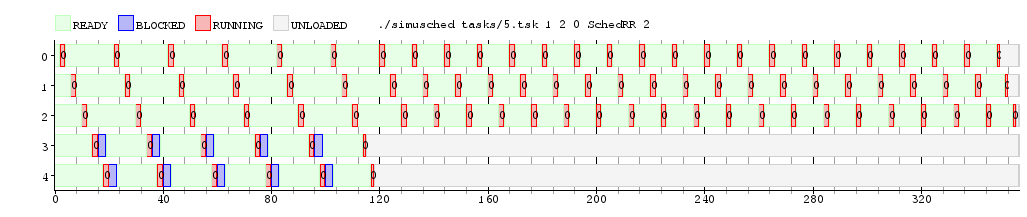
\includegraphics[width=\linewidth]{images/5_quantum2.png}
    \label{fig:Task Consola}
    \caption{Round-Robin (quantum=2)}
\end{figure}

\begin{figure}[h]
    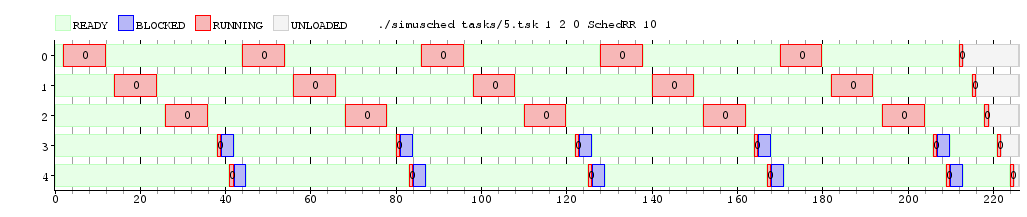
\includegraphics[width=\linewidth]{images/5_quantum10.png}
    \label{fig:Task Consola}
    \caption{Round-Robin (quantum=10)}
\end{figure}

\begin{figure}[h]
    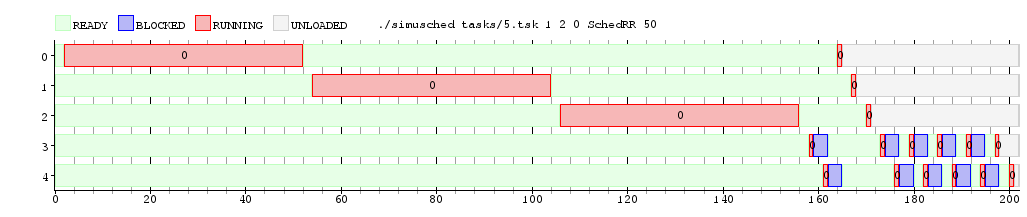
\includegraphics[width=\linewidth]{images/5_quantum50.png}
    \label{fig:Task Consola}
    \caption{Round-Robin (quantum=50)}
\end{figure}

En las 3 figuras anteriores podemos observar los diagramas de Gantt para el algoritmo del scheduler Round-Robin bajo el cual corre un mismo lote (el \textit{lote5}). En los 3 casos se trata de una CPU de un único núcleo, en el cual se tendrá un \textit{switch\_cost} de 2 ciclos de reloj. La particular diferencia entre los 3 es el \textit{quantum} pasado como parametro al Round-Robin, en el que su valor es de 2, 10, 50 respectivamente (según el orden de aparición). Este \textit{quantum} es el que determina cuantos ciclos le son lícitos a cada tarea permanecer en estado \textit{runing}. Ejecutando las tareas de manera alternada por el orden que rige una cola de tareas, cada vez que la CPU se encuentra disponible, se desencola la siguiente tarea y se vuelve a encolar aquella sin finalizar que haya agotado el \textit{quantum} de tiempo asignado. Para un \textit{quantum} no muy grande y tareas que requieran un tiempo no muy corto (menor que el \textit{quantum}), como es el escenario que figura en los 3 diagramas anteriores, el Round-Robin reduce las latencias, ya que al turnar de manera más \textit{justa} el volumen de tareas, la última no debe lidiar con la espera del tiempo completo de ejecución de sus predecesoras, como ocurre con el FCFS. No obstante, se distribuye un costo extra de intercambio de contexto, que repercute en un aumenta del tiempo total de ejecución del lote, de manera acorde a la frecuencia de conmutación dada por el \textit{quantum}. Experimentalmente esto se hace evidente en los graficos anteriores, en donde en el primer caso (el de menor \textit{quantum}) el lote abarca un tiempo significativamente mayor que el de los otros dos casos. A su vez el tercer caso, bajo un \textit{quantum = 50}, mejora levemente su performance contra su predecesor, de \textit{quantum = 10}. Sin embargo, no es buena idea tener un \textit{quantum} demasiado grande, pues la rutina tendería a degenerarse hacia el FCFS.
\newpage
\section{Comparacion Round-Robin/FCFS}

\subsection{FCFS}

El FCFS "First Come, First Served", como su nombre sugiere es un scheduler con una política de estilo FIFO, es decir que la primera tarea en la cola de tareas será la primera en pasar al estado \textit{runing} y la primera en finalizar (en el núcleo en el que fue asignada). Mas específicamente, dado como parametro el \textit{switch\_cost} y un número $n$ de cores, asigna las primeras $n$ tareas en estar en estado \textit{ready} a los $n$ núcleos disponibles (asignando la tarea \textit{IDLE} para aquellos para los cuales no haya alguna tarea lista), y permitiendoles permanecer en \textit{runing} sin conmutarlas con otras hasta que estas primeras finalicen; de modo que lidiada con cada tarea una sóla vez, y sin ningun tipo de desalojo intermedio. 

\subsection{Round-Robin}

El Round-Robin es un scheduler que consiste en asignarle un tiempo predeterminado llamado \textit{quantum} (recibido como parametro) a cada tarea de la cola de tareas para permanecer en estado \textit{runing}; finalizado este tiempo, si hay otras tareas en estado \textit{ready} esperando a ser ejecutaras, la tarea actual es desalojada y conmutada con la siguiente (en caso de no haber otra en la cola, sigue corriendo la actual). La tarea recién desalojada pasa a tomar el último lugar en la cola (si es que no había finalizado), teniendo que esperar a que el resto previamente encolado consuma el mismo \textit{quantum} de tiempo cada una. En caso de tratarse de una CPU con varios núcleos, la cola de tareas es desencolada a medida que se vaya desocupando algún núcleo (sin tener en cuenta para esto a la tarea \textit{IDLE}).

\subsubsection{Diagramas GANTT}

El siguiente diagrama fue generado con los siguientes parametros:

\begin{enumerate}
	\item lote\_tsk: 5.tsk
	\item num\_cores: 1
	\item switch\_cost: 2
	\item sched\_class: SchedFCFS
\end{enumerate}

\begin{figure}[h]
    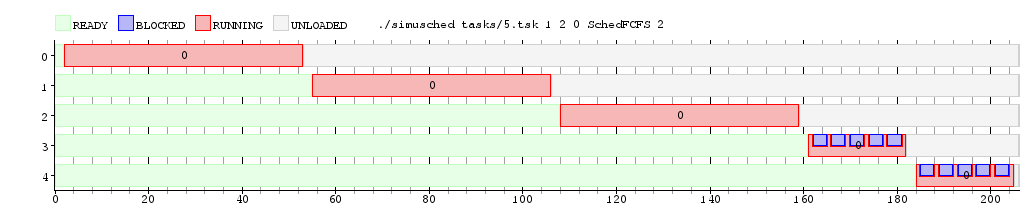
\includegraphics[width=\linewidth]{images/6_quantum2.png}
    \label{fig:Task Consola}
    \caption{FCFS}
\end{figure}

Ya hemos experimentado con este lote bajo el algoritmo de Round-Robin, y con diferentes \textit{quantums} durante el ejercicio anterior. Ahora en esta oportunidad lo hacemos bajo el algoritmo del scheduler FCFS, y con el mismo lote. La idea es exihibir las diferencias ya advertidas en ésta sección entre ambos schedulers. Para empezar como en el caso anterior, se requieren de 2 ciclos de reloj para cada intercambio de contexto, dandole este tiempo de espera a la primer tarea (de tipo TaskCPU). La diferencia mas notable con la rutina anterior es que cada tarea no es interrumpida sino hasta que la misma finalice, esto para ciertos lotes de tareas podría traer una penalización severa de performance, pues mientras una tarea realiza una llamada bloqueante, la CPU permanece ociosa hasta que la misma termine. Esta desventaja se hace mas grosera en aquellos casos en que el bloqueo se prolonga por mucho tiempo. Sin embargo en éste caso particular, como la mayoria de las tareas del lote son del tipo TaskCPU, el tiempo perdido en los bloqueos cortos de las otras dos tareas se compensan en ahorros de demora surgidos de la conmutación frecuente de tareas (cosa que ocurre en el Round-Robin), dando una performance parecida o hasta mejor que con el algoritmo de Round-Robin. Esta compensación es la responsable de que el FCFS aventaje al Round-Robin en este lote en particular; de hecho, en el ejercicio anterior, los resultados parecian indicar que en cuanto mas laxa la politica del Round-Robin se volviera, es decir cuanto mas grande sea el quantum, y por ende en mas \textit{parecido} fuese al FCFS, mejor sería su performance. No obstante es fácil encontrar casos en el que esto no ocurre, por ejemplo, en los casos en los que las tareas hagan varias llamadas bloqueantes de un tiempo suficientemente prolongado.
 En el caso del Round-Robin con \textit{quantum = 50}, el scheduller se comporta para las primeras 3 tareas casi como un FCFS (dejandolas correr casi en su totalidad sin interrupciones), para luego empezar a aprovechar su propiedad de conmutar tareas al realizarse llamadas bloqueantes, con lo que aprovecha algunos ciclos en los cuales en el FCFS la CPU estaría ociosa.
\newpage
\section{Mistery Scheduler}

A partir del \texttt{.o} de un scheduler, hicimos ingeniería inversa de su comportamiento a partir de la ejecución de varias instancias.

\subsection{Analisis}

Para tener una idea de lo que hace el scheduler probamos con los siguientes parametros:

\begin{enumerate}
	\item lote\_tsk: 2.tsk
	\item num\_cores: 1
	\item switch\_cost: 0
	\item sched\_class: SchedFCFS
	\item params: 5 6 7 8 9 10
\end{enumerate}

Primero ejecutamos las siguientes tareas

\begin{itemize}
	\item Tarea 0: 90 ciclos de CPU, 0 llamadas bloqueantes
	\item Tarea 1: 90 ciclos de CPU, 0 llamadas bloqueantes
	\item Tarea 2: 90 ciclos de CPU, 0 llamadas bloqueantes
\end{itemize}

El resultado fue el siguiente:

\begin{figure}[h]
    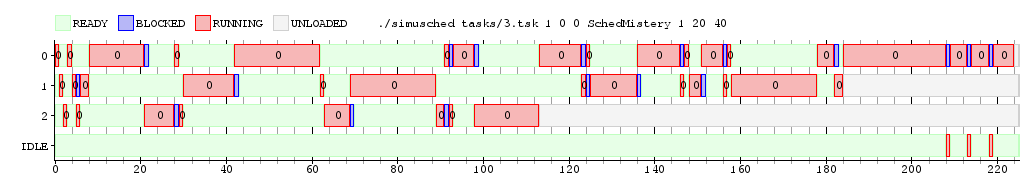
\includegraphics[width=\linewidth]{images/mist.png}
    \label{fig:Task Consola}
    \caption{Primera prueba}
\end{figure}

Aqui podemos apreciar que el scheduler tiene una cierta similitud con $Round Robin$, donde el quantum varia de manera rotativa segun los parametros pasados al scheduler. La primera vez que el proceso ejecuta lo hace por un ciclo y es desalojado, luego el quantum es determinado por los parametros recibidos hasta llegar al ultimo, a partir de ese momento el quantum es siempre el mismo hasta que el proceso termina de ejecutarse.

\pagebreak

Con esto en mente, procedimos a ver como operaba el scheduler con la incorporacion de tareas. Para esto se ejecutaron las siguientes tareas:

\begin{itemize}
	\item Tarea 0: 90 ciclos de CPU, 2 llamadas bloqueantes, incorporada en el momento 0
	\item Tarea 1: 90 ciclos de CPU, 4 llamadas bloqueantes, incorporada en el momento 20
	\item Tarea 2: 90 ciclos de CPU, 6 llamadas bloqueantes, incorporada en el momento 40
\end{itemize}

\begin{figure}[h]
    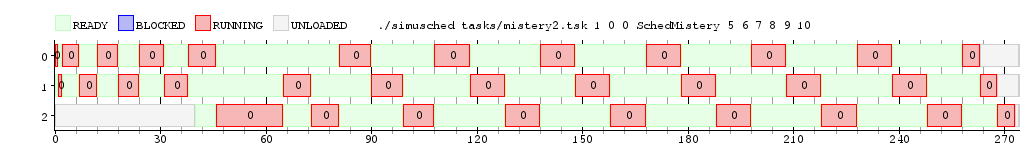
\includegraphics[width=\linewidth]{images/mist2.png}
    \label{fig:Task Consola}
    \caption{Segunda prueba}
\end{figure}

En este caso, al incorporar la tarea podemos observar que su quantum asignado es sumamente grande. Luego de mucho análisis observamos que en realidad estaba sumando los quantums que habíamos pasado por parámetro. Aquí es donde nos dimos cuenta que probablemente el Scheduler tenia múltiples colas con diferentes prioridades dadas por los parámetros de entrada. Siempre se ejecuta la tarea de máxima prioridad. La tarea 2 en un inicio se ejecuta por un quantum grande dado que se le suma el quantum de las colas de prioridad 1, 5, 6 y 7.

\hspace{2px}

Finalmente, buscamos ver como funcionaba el scheduler al incorporarse una tarea bloqueante.

\begin{figure}[h]
    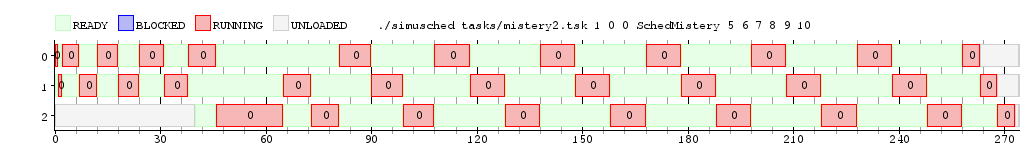
\includegraphics[width=\linewidth]{images/mist2.png}
    \label{fig:Task Consola}
    \caption{Tercera prueba \textbf{PONER LA POSTA}}
\end{figure}

Notamos que al entrar una tarea bloqueante seguía ejecutando la próxima de la cola y continuaba el Round Robin. Sin embargo, también notamos que al reincorporarse la tarea la misma tenia el quantum correspondiente a una cola con exactamente un nivel mayor de prioridad. De esta manera inferimos que al momento de reincorporar una tarea el scheduler si puede la asigna a una cola con un nivel mas de prioridad. A su vez, esto significa que en muchos casos esta sera la primera en ejecutarse al reincorporarse, sin tener que esperar al resto de las tareas que ya estaban en ejecucion.

\pagebreak

\subsection{Código}

\subsubsection{Class Declaration}
\begin{lstlisting}[language=C++, breaklines=true]
class SchedNoMistery : public SchedBase {
  public:
    SchedNoMistery(std::vector<int> argn);
    virtual void load(int pid);
    virtual void unblock(int pid);
    virtual int tick(int cpu, const enum Motivo m);
  private:
	std::vector<int> quantum_list;
	std::vector<std::queue<int> > q;
  std::map<int, int> blockedQueue;
	int cycles_left, current_queue, tasks;
	int next_pid(void);
};
\end{lstlisting}


\subsubsection{Constructor}
\begin{lstlisting}[language=C++, breaklines=true]
SchedNoMistery::SchedNoMistery(vector<int> argn) {
	// cpu cores, rest of params
	cycles_left = 1;
	current_queue = 0;
	tasks = 0;

	quantum_list.push_back(1);
	q.push_back(queue<int>());

	if (argn.size() > 1) {
		for (vector<int>::iterator it = ++argn.begin(); it != argn.end(); ++it) {
			quantum_list.push_back(*it);
			q.push_back(queue<int>());
		}
	}
}
\end{lstlisting}


\subsubsection{Load y Unblock}
\begin{lstlisting}[language=C++, breaklines=true]
void SchedNoMistery::load(int pid) {
	q.at(0).push(pid);
	tasks++;
}
\end{lstlisting}

\begin{lstlisting}[language=C++, breaklines=true]
void SchedNoMistery::unblock(int pid) {
	q.at(max(0,blockedQueue[pid]-1)).push(pid);
	blockedQueue.erase(pid);
	tasks++;
}
\end{lstlisting}


\subsubsection{Tick}
\begin{lstlisting}[language=C++, breaklines=true]
int SchedNoMistery::tick(int cpu, const enum Motivo m) {
	if (m == EXIT || m == BLOCK) {
		if (m == BLOCK) {
			blockedQueue[current_pid(cpu)] = current_queue;
		}
		
		tasks--;
		// current pid ended, get next
		if (tasks == 0) return IDLE_TASK;
		else { // get task from list
			return next_pid();
		}
	} else {
		if (current_pid(cpu) == IDLE_TASK && tasks > 0) {
			return next_pid();
		} else {
			cycles_left--;
			if (current_pid(cpu) != IDLE_TASK && cycles_left == 0) {

				current_queue = min(current_queue + 1, ((int) q.size()) - 1);
				if (tasks == 0) {
					cycles_left = quantum_list.at(current_queue);
					return current_pid(cpu);
				} else {
					q.at(current_queue).push(current_pid(cpu));
					return next_pid();
				}
			}
			return current_pid(cpu);
		}
	}
}

/* Requires some queue not to be empty */
int SchedNoMistery::next_pid() {
	int selectQueue = 0;
	for (vector<queue<int> >::iterator it = q.begin(); it != q.end(); ++it) {
		if ((*it).size() > 0) break;
		selectQueue++;
	}
	int pid = q.at(selectQueue).front();
	q.at(selectQueue).pop();
	current_queue = selectQueue;
	cycles_left = quantum_list.at(selectQueue);
	return pid;
}

\end{lstlisting}

\pagebreak

\textbf{BORRAR LO SIGUIENTE?}

\subsection{Diagramas y analisis del scheduler}
Para poder analizar el comportamiento del scheduler, decidimos armar el siguiente lote de tareas:

\begin{lstlisting}
	*3 TaskCPU 10
@4
*3 TaskCPU 5

TaskConsola 2 1 4
TaskConsola 5 1 1
TaskConsola 10 1 2
*3 TaskCPU 10
@20:
TaskCPU 10
\end{lstlisting}

De este gráfico podemos inferir lo siguiente:

\begin{itemize}
	\item El scheduler es un round robin con algunas particularidades
	\item Al incoporarse una nueva tarea, se la coloca en el tope de la cola del scheduler.
\end{itemize}

Este ultimo punto es importante, si dos tareas se incoporan durante la ejecucion de otra tarea, primero concluye el quantum de la tarea actual y se procede a cambiar la tarea con la primera que llego. Es por esta razon que elegimos implementar el scheduler sobre una lista, ya que nos permite agregar los elementos en las posiciones que precisamos.

Otra cosa que determinamos mediante experimentacion, es que el scheduler toma una cantidad arbitraria de parametros. Despues de varias pruebas, pudimos determinar el comportamiento del scheduler respecto a los parametros. Si tomamos los parametros \texttt{5 4 3 2 1}, todas las tareas van a ejecutarse por primera vez con un quantum de un ciclo (esto es independiente de los parametros). Posteriormente el scheduler toma los valores del quantum a partir de los parametros del scheduler de forma ordenada y ciclica, es decir, el quantum de una tarea seria \texttt{1}, \texttt{5}, \texttt{4}, \texttt{3} ,\texttt{2}, \texttt{1}, \texttt{5}, \texttt{4} y asi sucesivamente hasta que concluye la ejecucion de la tarea.

Por ultimo, esta el analisis como responde el scheduler ante las llamadas bloqueantes. Si una tarea tiene una llamada bloqueante se procede a desalojarla hasta que la misma se resuelve, una vez que se resuelve se procede a agregarla nuevamente a la lista con un quantum de un ciclo. Esto ocurre independientemente de los parametros que recibe el scheduler.
\newpage
\section{Round Robin 2}

Para la implementacion de $Round Robin 2$ se utilizo como base la implementacion original de $Round Robin$, a partir de esta se modifico segun los nuevos requerimientos.

\subsection{Codigo}

\subsubsection{Class Declaration}
\begin{lstlisting}[language=C++, breaklines=true]
class SchedRR2 : public SchedBase {
	public:
		SchedRR2(std::vector<int> argn);
        ~SchedRR2();
		virtual void load(int pid);
		virtual void unblock(int pid);
		virtual int tick(int cpu, const enum Motivo m);
	private:
		int* quantum;
		int* cycles;
		std::vector<std::queue<int> > q;
		std::vector<int> totalLoad; // buscar otra estructura?
		std::map<int,int> CPUBlockedTask;

		int getCPU();
};
\end{lstlisting}

A diferencia de $Round Robin$, en este caso tenemos una cola de tareas por CPU, la carga total por procesador y un $map$ que sirve para tomar nota de los procesos bloqueados y del procesador que tiene asingado.

\subsubsection{Constructor y Destructor}
\begin{lstlisting}[language=C++, breaklines=true]
SchedRR2::SchedRR2(vector<int> argn) {
	// Round robin recibe la cantidad de cores y sus cpu_quantum por parametro
	quantum = new int[argn.size()-1];

	for (int i = 0; i < argn[0]; ++i) {
		q.push_back(queue<int>());
		totalLoad.push_back(0);
	}

	for (int i = 1; i < (int) argn.size(); i++) {
		quantum[i-1] = argn[i];
	}

	cycles = new int[argn[0]];
}

SchedRR2::~SchedRR2() {
	delete[] cycles;
	delete[] quantum;
}
\end{lstlisting}

Aqui inicalizamos las estructuras de datos utlizando los parametros recibidos, inicialmente la carga es cero para todos los procesadores.

\subsubsection{Load y Unblock}
\begin{lstlisting}[language=C++, breaklines=true]
void SchedRR2::load(int pid) {
	int cpu = getCPU();
	q.at(cpu).push(pid);
	totalLoad[cpu]++;
}

void SchedRR2::unblock(int pid) {
	q.at(CPUBlockedTask[pid]).push(pid);
}

int SchedRR2::getCPU() {
	int cpu = 0;
	int i = 1;
	for (vector<int>::iterator it = ++totalLoad.begin() ; it != totalLoad.end(); ++it) {
		if (*it < totalLoad.at(cpu)) {
			cpu = i;
		}
		i++;
	}
	return cpu;
}
\end{lstlisting}

En el caso del $load$ tenemos que buscar la CPU que tenga menor carga total, para hacer esto contamos con la funcion auxiliar \texttt{getCPU()} la cual se encarga de recorrer el vector \texttt{totalLoad} en busca del procesador adecuado. Una vez obtenida dicha CPU, procedemos a agregar la tarea a su cola y aumentamos la carga total en uno.

En el caso del $unblock$ hacemos uso del $map$, simplemente volvemos a agregar la tarea a la CPU donde se produjo la llamada bloqueante, ya que la tarea necesita haber estado bloqueada para llamar a $unblock$ el $map$ siempre va a dar una CPU valida.

\subsubsection{Tick}
\begin{lstlisting}[language=C++, breaklines=true]
int SchedRR2::tick(int cpu, const enum Motivo m) {
	if (m == EXIT || m == BLOCK) {
		// Si la tarea termino, se la quita de la carga total.
		// Si se bloqueo, se toma nota de la CPU actual para poder
		// agregarla nuevamente cuando se desbloquee.
		if (m == EXIT) {
			totalLoad[cpu]--;
		} else {
			CPUBlockedTask[current_pid(cpu)] = cpu;
		}

		// Si el pid actual termino, sigue el proximo.
		if (q.at(cpu).empty()) return IDLE_TASK;
		else {
			int sig = q.at(cpu).front(); q.at(cpu).pop();
			cycles[cpu] = quantum[cpu];
			return sig;
		}
	} else {
		if (current_pid(cpu) == IDLE_TASK && !q.at(cpu).empty()) {
			int sig = q.at(cpu).front(); q.at(cpu).pop();
			cycles[cpu] = quantum[cpu];
			return sig;
		} else {
			cycles[cpu]--;

			if (cycles[cpu] == 0) {
				if (q.at(cpu).empty()) {
					cycles[cpu] = quantum[cpu];
					return current_pid(cpu);
				} else {
					int sig = q.at(cpu).front(); q.at(cpu).pop();
					q.at(cpu).push(current_pid(cpu)); // re-add to queue
					cycles[cpu] = quantum[cpu];
					return sig;
				}
			} else {
				return current_pid(cpu);
			}
		}
	}
}
\end{lstlisting}

El $tick$ opera de manera casi identica a la del de $Round Robin$, la unica diferencia es la cola de tareas individual por CPU, como manipular los bloqueos y el fin de las tareas.

Si el $tick$ es normal (es decir, no es un bloqueo ni un fin de ejecucion), se procede igual que $Round Robin$, con la diferencia que en vez de usar la cola global \texttt{q} usamos la cola correspondiente a la CPU actual. Si por el contrario recibimos un \texttt{BLOCK} guardamos la CPU del proceso actual en el $map$, en el caso de \texttt{EXIT} procedemos a reducir la carga del CPU actual en uno, en ambos casos luego procedemos a desalojar la tarea, cargar la siguiente (si es que la hay) y resetear el quantum.

\subsection{Lote de tareas de prueba}

Para ver el beneficio de la migracion de proceso, vamos a probar con las siguientes tareas:

\begin{itemize}
	\item Tarea 0: 100 ciclos de CPU, 0 llamadas bloqueantes
	\item Tarea 1: 50 ciclos de CPU, 0 llamadas bloqueantes
	\item Tarea 2: 100 ciclos de CPU, 0 llamada bloqueante
	\item Tarea 3: 50 ciclos de CPU, 0 llamadas bloqueantes
	\item Tarea 4: 100 ciclos de CPU, 0 llamadas bloqueantes
\end{itemize}

\begin{figure}[h]
    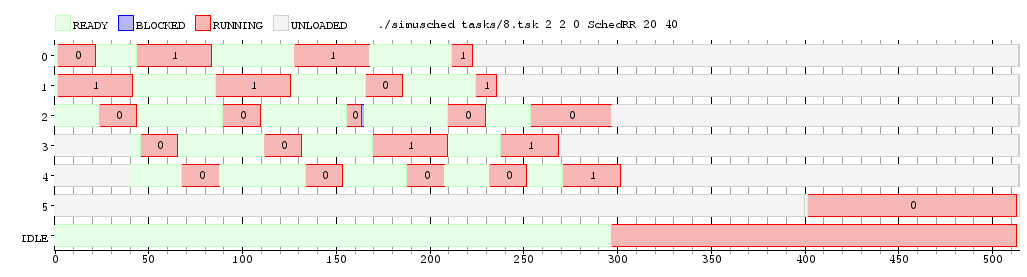
\includegraphics[width=\linewidth]{images/8_quantumRR.png}
    \label{fig:Task Consola}
    \caption{Round Robin}
\end{figure}

\begin{figure}[h]
    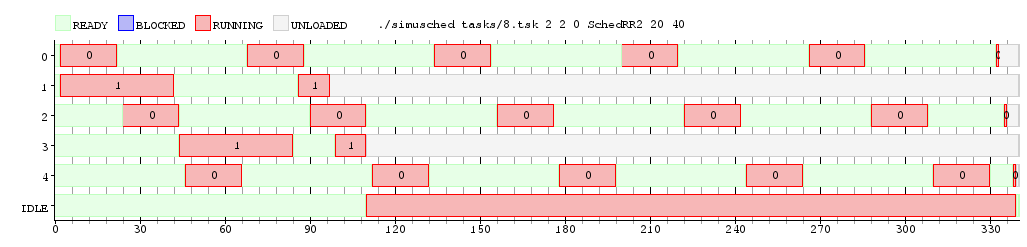
\includegraphics[width=\linewidth]{images/8_quantumRR2.png}
    \label{fig:Task Consola}
    \caption{Round Robin 2}
\end{figure}

\pagebreak

En este caso podemos ver claramente que la migracion de procesos entre nucleos ayuda a reducir ampliamente el tiempo total en el sistema de varias tareas. Debido a nuestra implementacion, los procesos que toman 100 ciclos van a parar a la primer CPU, mientras que los que toman 50 ciclos son asignados a la segunda CPU. Con respecto a temas de $latencia$, podemos ver que $Round Robin 2$ tiene mejor comportamiento que $Round Robin$, sin embargo, esta distribucion de tarea impacata negativamente a la concurrencia ya que una vez concluidas las tareas 1 y 3, la segunda CPU entra en estado oscioso y el scheduler no le asigna mas procesos. Esto ultimo hace que la ultima tarea concluya aproximadamente a los 230 ciclos en el caso de $Round Robin$, mientras que en $Round Robin 2$ la ultima tarea concluye aproximadamente a los 340 ciclos.

Para ver un caso donde la migracion de procesos no mejora significativamente los tiempos totales de ejecucion, tenemos el siguiente caso:

\begin{itemize}
	\item Tarea 0: 100 ciclos de CPU, 0 llamadas bloqueantes
	\item Tarea 1: 50 ciclos de CPU, 50 llamadas bloqueantes
	\item Tarea 2: 100 ciclos de CPU, 0 llamada bloqueante
	\item Tarea 3: 50 ciclos de CPU, 50 llamadas bloqueantes
	\item Tarea 4: 100 ciclos de CPU, 0 llamadas bloqueantes
\end{itemize}

\begin{figure}[h]
    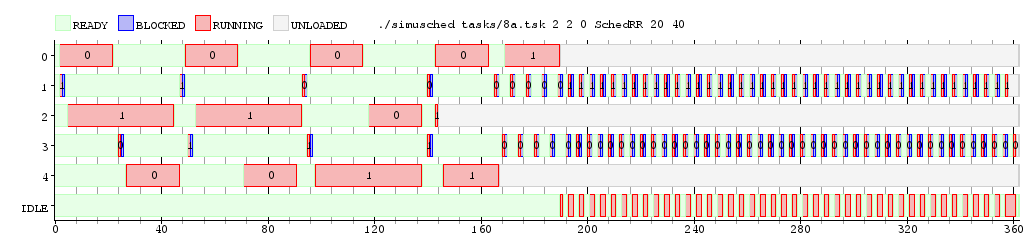
\includegraphics[width=\linewidth]{images/8a_quantumRR.png}
    \label{fig:Task Consola}
    \caption{Round Robin}
\end{figure}

\pagebreak

\begin{figure}[h]
    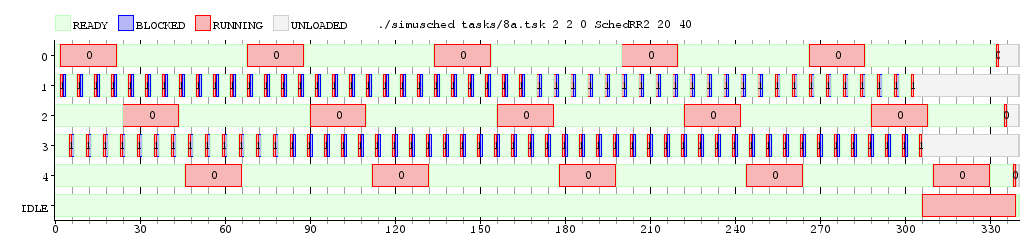
\includegraphics[width=\linewidth]{images/8a_quantumRR2.png}
    \label{fig:Task Consola}
    \caption{Round Robin 2}
\end{figure}

Aqui podemos apreciar que la migracion de procesos entre nucleos no nos aporta una mejora significativa, la cantidad de llamadas bloqueantes es suficientemente grande como para nulificar cualquier tipo de beneficio de la migracion entre procesos. Incluso podemos apreciar que la migracion hace que si bien algunas tareas concluyan en menor tiempo, durante una gran cantidad de tiempo tenemos algun nucleo en estado oscioso en el caso de $Round Robin$.

\newpage

%\section{Codigo}
%\subsection{matrix.h}
%\lstinputlisting[language=C++, breaklines=true]{../src/src/matrix.h}

\end{document}